\section{Dos au Muur}
On attaque ici le cinquième et dernier chapitre de la saga.

\subsection{Résumé des épisodes précédents}
Le camp opposé (l’empire pour les gentils et l’alliance si vos héros sont avec Dark Vador) a récupéré l’\nameref{sec:oubliette-de-dreypa} au nez et à la barbe de vos héros qui sont donc bien dégouttés. S’ils ont bien joué, vos héros ont trouvé l’Holocron de Muur dans le laboratoire de \nameref{sec:pulsipher}. Et enfin, vos héros savent ce que contient l’oubliette.

Ils vont donc errer un moment dans l’Univers à la recherche d’informations qui pourraient les mener à l’oubliette perdue. Selon que vos joueurs se montrent imaginatif ou non dans leurs investigations, vous pourrez abréger la séquence par un appel de leur hiérarchie qui souhaitera leur faire part d’une information. Si vos joueurs se montrent imaginatif faites leur trouver la dite information par eux-mêmes.

\subsection{Sur la piste}
\paragraph{Empire}
Si vos héros sont à la solde de l’Empire, l’information qui finie par leur parvenir est que des espions infiltrés ont découvert au péril de leur vie que les rebelles ont amené sur une base reculée de l’alliance, une cargaison très spéciale et que depuis, seul le personnel fortement accrédité est autorisé à circuler dans la zone de stockage de la cargaison.

La base rebelle se trouve sur la lune IV de Yavin. Les rebelles sont établis dans ce système depuis plusieurs mois. La quatrième lune de Yavin est une lune forestière avec une végétation dense offrant un bon camouflage aux bâtiments installés sous la canopée. La lune possède plusieurs installations distante les unes des autres de plusieurs centaines de kilomètres. La fameuse cargaison est entreposée, et sans doute étudiée, dans l’installation la plus au Nord et la plus éloignée de toutes les autres.

\paragraph{Alliance}
Si vos héros se sont enrôlés dans la résistance, c’est un peu la même histoire. L’information qui leur parvient est que l’Empire à fait porter sur une lune de Lothal une cargaison et que depuis, le bâtiment où est entreposée la cargaison est verrouillé. 

Sur l’une des lunes de Lothal, l’Empire possède une base militaire. La lune est de type désertique. Pas de végétation ni d’eau, seulement une atmosphère un peu raréfiée. La cargaison est entreposée 100~km au Nord de la base dans une zone qui depuis est fermée à tous le personnel non autorisés.

\paragraph{Commun}
Dans tous les cas, les héros sont prévenus que le camp adverse s’emploie à ouvrir l’Oubliette mais que, pour l’instant, il n’y est pas parvenu.

\'A ce moment de l’histoire, vos héros devraient sentir (ou non) le piège, il leur faut donc un plan. Ils savent que dans l’oubliette se trouve \nameref{sec:celeste-morne}, une puissante Jedi et, qui plus est, possédée par le Talisman de Muur, un non moins puissant Sith ! Le combat, si combat il doit y avoir, s’annonce un peu difficile. \'A vous de leur faire comprendre, s’ils ne le ressentent pas spontanément, qu’y allez sans un plan pour libérer Céleste du Talisman n’est rien de plus qu’un suicide collectif.

\subsection{Man with a plan}
C’est là qu’intervient l’Holocron de Muur.

S’ils ne l’ont pas trouvé, hé bien c’est qu’ils ont mal joué ! La meilleure solution est encore de leur faire comprendre qu’il leur manque une pièce du puzzle et qu’ils doivent retourner sur \nameref{sec:jebble} chercher l’Holocron. Par exemple en leur rappelant que le datapad de \nameref{sec:pulsipher} faisait référence à un objet triangulaire.

S’ils ont l’Holocron avec eux, il est temps de laisser entendre que c’est un élément important de l’histoire et qu’il va falloir trouver comment l’ouvrir. Pour l’ouvrir ils vont devoir retourner sur \nameref{sec:taris} dans les ruines de l’ancien temple Sith. 

\begin{samepage}
\begin{paperbox}{Comment les amener sur Taris ?}
    Quelques idées sur comment les amener à retourner sur Taris pour ouvrir l’Holocron. Car ce dernier étant verrouillé sur l’esprit de Muur, il n’est pas possible de l’ouvrir, même pour un apprenti Sith.

    \begin{rebelist}
        \item S’il y a un héros sensible à la Force parmi les joueurs, le plus simple est de lui donner une vision dans laquelle il voit le monolithe. Ou plus subtil, il voit les mêmes évènements que ceux décrit par le Monolithe.
        \item Sinon, \nameref{sec:garan-keggle} ou \nameref{sec:dass-jennir} peuvent aider. En expliquant aux héros que les holocrons qui sont comme celui-là verrouillé sur l’esprit de leur propriétaire, ont souvent une clé physique permettant de ne pas perdre le savoir une fois le propriétaire décédé. C’est, en général, un lieu ou un objet fortement lié à ce dernier, duquel émane une Force caractéristique (comme le Monolithe).
    \end{rebelist}
\end{paperbox}
\end{samepage}

\paragraph{(optionnel Alliance) Infiltration sur Taris}
\textit{Selon vos joueurs, il se peut que leur départ de Taris ait été un peu mouvementé. Et même sans ça, ça commence à faire plusieurs mois qu’ils mettent le bordel dans les affaires de l’Empire qui a commencé à les rechercher. Du coup ils ne peuvent pas se poser sur Taris comme des fleurs et espérer qu’on leur ouvre la route jusqu’au temple. Voici ce que mes joueurs ont fait.}\\ 

Ils ont décidé de voler des uniformes de \nameref{sec:storm-trooper}. \nameref{sec:lindi-dangon} leur a donné la position d’un contingent de \nameref{sec:storm-trooper} repéré sur une lune pas lion de leur position. Les héros s’y rendent donc pour voler des uniformes et plus si possible.

Sur place voir le \nameref{fig:storm-troopers-camp} est composé d’une vingtaine de soldats, pas plus de 10 sont visibles, le reste est dans les tentes. Le camp est fortifié et protégé par deux \nameref{sec:at-st} et une batterie de canon anti-aérien.\\ 
\'A environ 500~m à l’Est du camp se trouve stationner 2 navettes de transport impériale, gardé par 2x 3 \nameref{sec:storm-trooper}s.

Le but est dans de récupérer une armure par héros voire d’embarquer une navette pour se poser sans encombre sur Taris. Le camp est très bien gardé, tenté une infiltration à plus de chance de fonctionner qu’un passage en force.

\paragraph{(optionnel Empire) Repousser les rebels}
Histoire de garder un équilibre Alliance / Empire, si vos joueurs sont à la solde de l’Empire et s’ennuient un peu, vous pouvez, lors de leur arrivée sur Taris, plutôt que de les diriger vers le spatioport, les emmener vers un campement de l’Empire, plus pratique pour eux et plus proche du temple (c’est \nameref{sec:garan-keggle} qui le dit).

Sur place voir le \nameref{fig:storm-troopers-camp}, ils poseront leur vaisseau sur l’emplacement libre. Et à peine descendu, un escadron de rebelle se jette sur eux, ils semble qu’ils en ai après le vaisseau stationné à coté du leur\ldots

\paragraph{Holocron ouvre-toi}
Une fois de retour dans le temple, sur le Monolithe en y regardant d’un peu plus prêt on trouvera un emplacement triangulaire où l’Holocron entre à la perfection. Placer dans cette serrure, l’Holocron s’ouvre et libère ses secrets. C’est un mélange de visuel et de perceptions mentale, les héros sensibles à la Force comprennent mieux ce qu’ils voient, les autres font un jet de \textit{Vigueur+2} pour ne pas s’évanouir.

\noindent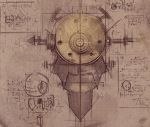
\includegraphics[width=\linewidth]{_img/talisman-book.png}

On voit (et on ressent) \nameref{fig:karness-muur} en train de concevoir l’artefact, étape par étape. Un jet de \textit{Connaissance (Force)} pour les héros possédant l’Atout \textit{Jedi} ou \textit{Sith} permet à ce dernier de comprendre ce que Muur est en train de faire.

Néanmoins, tous ceux qui ne se sont pas évanoui remarquent et ressentent quelque chose en assistant à la fabrication du Talisman. Ce dernier n’est pas parfait, Muur n’a fait qu’un seul essai et il a été hésitant lors de certaines étapes. Le Talisman a donc de grandes chances de posséder des micro-fissures, suffisantes même pour le détruire à condition de posséder un pouvoir immense, au-delà même de celui d’un simple Jedi. Mais il est probable qu’un impact avec un projectile ou un sabre, chargé de Force, étire les fissures suffisamment pour que l’hôte, au prix d’un effort considérable, parvienne à reprendre le dessus et se libère du Talisman.

Dans ce cas, pendant un court laps de temps, il serait possible de détacher l’artefact et de le jeter dans l’oubliette. L’ancien hôte demeurerait toutefois incapable de se défendre et vidé de ses forces pendant un moment.

\subsection{La bataille finale}
Avec leur plan en tête vos héros partent donc pour la bataille finale, sur la lune de Lothal/Yavin (selon leur camp). Ils ont les coordonnées approximatives de la zone de test où se trouve l’oubliette. 

Dès qu’ils survolent la zone, un Force inconnue attire le Nimbus au sol et l’oblige à se poser. Les héros se retrouvent dans une sorte de cratère, tout autour d’eux, des centaines de Rakghouls sont rassemblés. Au loin, à pas loin d’1~km se trouve Céleste Moorne qui les regarde. Manifestement, l’oubliette a été ouverte !

Avant qu’ils n’aient eu le temps d’y réfléchir, une première vague de \nameref{sec:rakghoul}s (prévoir 10 / 12) se dirige vers eux à grande vitesse. Ils peuvent se servir des canons du vaisseau pour éliminer la première vague. Une fois la première vague éliminé, il ne se passe rien tant qu’ils ne sortent pas du vaisseau. Ils ne peuvent pas faire redécoller le vaisseau. S’ils ne parviennent pas à éliminer la première vague en 50 tours, les Rakghouls pénètrent dans le vaisseau, il faudra les finir à la main.

Une fois sorti du vaisseau, la deuxième vague de \nameref{sec:rakghoul}s (prévoir 1.5 Rakghoul par héros) s’élance vers eux tandis que Céleste se contente d’observer de loin. Laissez les héros engager le combat, s’ils ne s’en sortent pas ou quand il ne reste qu’1 ou 2 ennemis, lancer une nouvelle vague, massive cette fois avec des \nameref{sec:rakghoul-amblyope} en prime, ça arrive de tout les côtés. Il faut que vos joueurs sentent leur fin proche. 

\paragraph{Résistance}
Puis quand ils ont bien paniqué, l’Uhumele sort de la couche nuageuse et commence à canarder dans tous les sens sur les Rakghouls. Et là, c’est Dass Jennir qui saute du vaisseau et qui vient se placer au côté des héros, suivit de tout l’équipage de \nameref{sec:schurk-heren}. 
\begin{quotebox}
    \nameref{sec:dass-jennir}: On s’occupe de vous ouvrir la voie, faite ce que vous devez faire !
\end{quotebox}

\paragraph{Empire}
Puis quand ils ont bien paniqué, un Croiseur léger de l’Empire sort de la couche nuageuse et commence à canarder dans tous les sens sur les Rakghouls. Et là, c’est \nameref{sec:garan-keggle} qui saute du vaisseau et qui vient se placer au côté des héros, suivit d’un contingent de \nameref{sec:storm-trooper}. 
\begin{quotebox}
    \nameref{sec:garan-keggle}: On s’occupe de vous ouvrir la voie, faite ce que vous devez faire !
\end{quotebox}

\paragraph{Commun}
La bataille fait rage, ça part dans tous les sens, les héros avancent péniblement vers Céleste, de temps à autre faite un lancer de dés, si plus de 4, les héros se trouvent face à face avec autant de Rakghouls que le dé dépasse 4 (Ex: 6 = 2 Rakghouls). Ils sont alors obligés de les affronter.

Après moult batailles, les héros se retrouvent face à Céleste Morne, possédé par l’esprit de Muur qui s’adresse aux héros qui devront faire un jet d’\textif{\'Ame} pour résister à l’Intimidation. 
\begin{quotebox}
    \nameref{fig:karness-muur}: Ah Ah Ah ! Vous pensez vraiment pourvoir m’arrêter ? Vous n’êtes que des insectes face à mon Pouvoir !
\end{quotebox}
    Puis soudain Céleste semble parcouru d’un spasme. Son visage se crispe. Elle semble se battre contre un démon intérieur \ldot
\begin{quotebox}
    \nameref{sec:celeste-morne}: Fuyez vous ne pourrez pas le maîtriser ... 
\end{quotebox}

C’est alors que commence la phase de combat. \'A chaque tour, Céleste fait un jet \textit{d’\^Ame}, si le jet est raté, Karness attaque, si le jet est réussit, Céleste parvient à le retenir, en cas de relance, Karness est secoué pour le prochain tour.

Les héros doivent charger une arme (Sabre Laser ou Phaser) avec la Force. S’il n’y a personne de sensible à la Force dans le groupe, faite venir \nameref{sec:dass-jennir} ou \nameref{sec:garan-keggle} avec eux jusqu’à Céleste afin de charger l’arme.

Peu importe qui charge l’arme, il ne pourra rien faire d’autre pendant son tour. Pour charger l’arme il doit réussir 2 jets de \textit{Maîtrise de la Force}.

Ensuite il faudra que quelqu’un (l’un des héros PJ) utilise l’arme et réussisse l’action. S’il touche c’est gagné, s’il rate, il faut recommencer. En attendant, les héros sont confrontés à Karness ou à de petits groupes de Rakghouls. Si les héros frappent Céleste trop facilement, faite leur frapper un deuxième coup pour que ça fonctionne. Si Karness n’est pas secoué lors de l’attaque, le fait de visé le Talisman augmente la difficulté d’un Tir de \textbf{2}.

\subsection{Epilogue}
Le Talisman est touché, Céleste se met à hurler et une vague de Force Lumineuse part de son corps et s’étend sur l’ensemble du cratère. Les Rakghouls touchés par cette vague perdent toute cohésion et combativité. Le Talisman se détache alors du bras de Céleste et tombe à terre en même temps que Céleste s’écroule au sol, en quelques secondes son corps se met à vieillir jusqu’à se décomposer en poussière. Le Talisman la maintenait en vie depuis plus de 1000~ans.

\noindent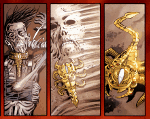
\includegraphics[width=\linewidth]{_img/pnjs/celeste-morne-death.png}

L’oubliette se trouve à 200~m derrière Céleste, c’est à vos héros de voir ce qu’ils font. Mais s’ils ne font rien dans les 2~mn, le Talisman va s’accrocher à \nameref{sec:dass-jennir} ou \nameref{sec:garan-keggle} et dans ce cas tout est perdu. Normalement ils devraient balancer le Talisman dans l’oubliette et refermer.

Bon là c’est la méga-happy-end à vous de voir.

\subsubsection{Progression}
Les héros reçoivent 4~XP pour ce scénario. Ils reçoivent aussi un Atout \textit{Contact} en la personne de \nameref{sec:dass-jennir} ou \nameref{sec:garan-keggle} qui les appréciera pour les qualités dont ils ont fait preuve dans cette mission.

\begin{wrapfigure}{R}{180pt}
    \centering
    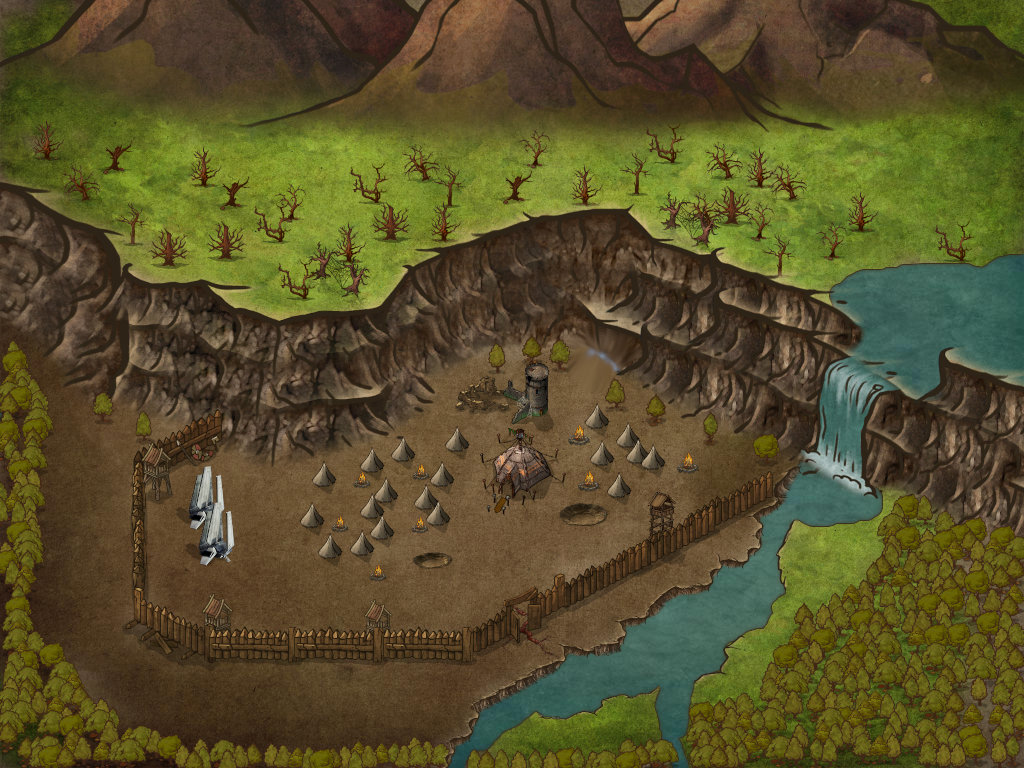
\includegraphics[width=180pt]{_img/place/storm-troopers-camp.png}
    \caption{\label{fig:storm-troopers-camp}Camp de Storm Troopers}
\end{wrapfigure}